\documentclass[twoside,english, a4paper]{article}
\usepackage{graphicx}
\usepackage{amssymb,amsmath}
\usepackage{color}

\definecolor{MinSig}{RGB}{255,163,53}
%~ \definecolor{MinSig}{RGB}{199,154,0}
\newcommand{\highlightMinSig}[1]{\textcolor{MinSig}{\bf{#1}}}

%~ \newcommand{\mathbox}[1]{\fbox{\begin{minipage}{\linewidth}#1\end{minipage}}}
\newcommand{\mathbox}[1]{#1}

\title{\textsc{Dnssec} Key State Transitions \\ \small The Grand Unified Theory of Everything \textsc{Dnssec} ;)}
\author{Yuri Schaeffer, Yuri@NLnetLabs.nl}
\date{\today}

\setcounter{tocdepth}{2}

\begin{document}
\maketitle
\tableofcontents

\section{Introduction}

During a key roll over each involved key has a state. Matthijs 
Mekking pointed out that the state-machine for this key can be 
represented as three individual smaller state machines: The state at 
the parent, the private key state, and the public key state. 

That idea is the basis for this document. A cache centered rather 
than a roll-over centered approach is chosen and the three different 
state machines are generalized to one type of state machine. The three
state machines now represent the public records associated with a key 
(\textsc{ds}, \textsc{dnskey}, \textsc{rrsig}). The state of each record is defined by its 
reputation among all DNS caches in the world. 

With this we are able to formalize the boundaries of DNSSEC and make
precise statements about the validity of a zone with respect to DNSSEC.
This has two levels: One of them is that we can judge any invariant of
states on validity. The other is that for each state we know under
what exact circumstances we can me a transition to the next state.

\section{Cache Centered Approach}

The cache centered approach uses a few extra concepts. Each key has 
a goal, an internal desire to be either known to all caches around 
the world or no caches at all. A system can make any state 
transition as long as it makes sure that the validity of a zone in 
general is not compromised. This does also imply that a key's goal can
be changed at any time without the zone going bogus. E.g. if a key has
a desire to disappear but is the only key left it will stay on duty for
as long as necessary. Also, new keys can be introduced at any time.

Using a cache centered approach has a number of advantages. Here, in 
contrast to a roll-over centered approach, keys have no direct 
relation to each other. The system does not try to roll from one 
specific key to another specific key but rather satisfy all goals 
while remaining valid as a whole. Essentially the roll-over is a side 
effect of the strive to satisfy key goals. New keys can be 
introduced and goals can be redefined at any time without a problem. 
This makes the system agile, robust, and capable of handling unexpected
situations.

This point of view makes sense since the identities validating the 
zone are viewing it from a cache's perspective. We only have to make 
sure every
possible view on the data is valid at any point in time.

\subsection{Key States} \label{sec:keystates}

A key has two pieces of public information which are 
represented by three resource records: DS, DNSKEY, and RRSIG. Each of 
which can be known to a different set of caches and thus require their
own state machine (Figure~\ref{fig:states}). When we say a key has 
goal \emph{X} we mean that it wants to move all its records to state
\emph{X}.

\begin{figure}[h]
	\centering
	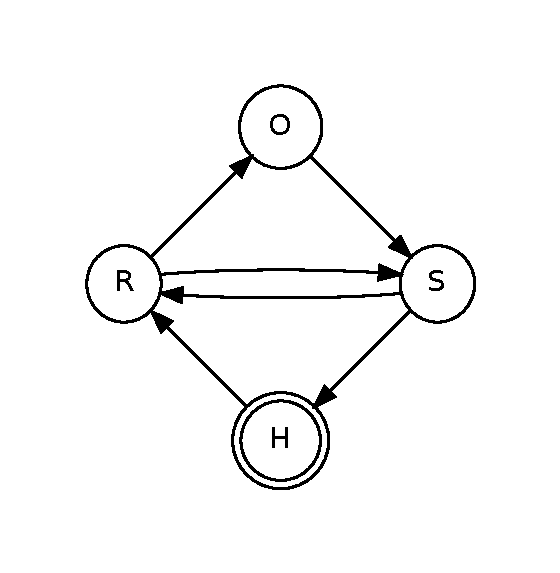
\includegraphics[scale=0.5]{states.pdf}
	\caption{State diagram for individual records.}
	\label{fig:states}
\end{figure}

The state of a resource record is defined by its reputation in 
world's caches. There are 2 certain states, \emph{Hidden} and \emph
{Omnipresent}. In the first state a resource record is not available 
in any cache (anymore). Similarly in the latter state we are sure 
all caches have a copy of the record or can at least obtain it (i.e. 
they have no old unexpired resource record set).

The two other states represent uncertainty: \emph{Rumoured} and \emph
{Squashed}. The separation is a bit artificial as they more or less 
mean the same. Both represent that some caches do and some don't 
know about the resource record. However, in our model actions (which 
are observable by the outside world) are only taken on state 
transitions. If the goal of a key changes while a record is in an 
uncertain state the records reputation does not immediately change. We 
do however must explicitly tell the component responsible for 
publishing the record to introduce or withdraw it. 
%~ This transition 
%~ is represented by the dashed arrow in Figure~\ref{fig:states}.

Since DNS involves caches and TTLs, it is entirely possible for a 
record being in the \emph{Rumoured} state while in fact every cache 
in the world holds the record. The problem is the uncertainty, we have
no way to know a record is fully propagated other than waiting the
worst case propagation time. This is also true for the \emph{Squashed}
state.

\paragraph{Summary.} A record is always in one of these four states:

\begin{itemize}
       \item[\emph{Hidden}:] 		
			The record is in no cache at all.
       \item[\emph{Rumoured}:] 		
			The record is published but not every cache might be aware.
\item[\emph{Omnipresent}:]
			Every cache has this record.
			Or (Section~\ref{redifined-propagated}) a
			sibling record.
\item[\emph{Squashed}:]
			The record is withdrawn but some caches might still have it.
\end{itemize} 

\paragraph{Formal definition of record states.} Let $r$ be a record, $Anounced$ the 
collection of records that are actively published, and $\mathbb{C}$
the collection of all caches in the world. The states are defined by:

\begin{displaymath}
\begin{array}{lllll}
       r\in Hidden      & \equiv & H(r) &=& \forall c \in \mathbb{C} \cdot r \not \in c \\
       r\in Rumoured    & \equiv & R(r) &=& \exists c \in \mathbb{C} \cdot r \not \in c \wedge \exists c \in \mathbb{C} \cdot r\in c \wedge r\in Announced\\
       r\in Omnipresent & \equiv & O(r) &=& \forall c \in \mathbb{C} \cdot r \in c \\
       r\in Squashed    & \equiv & S(r) &=& \exists c \in \mathbb{C} \cdot r \not \in c \wedge \exists c \in \mathbb{C} \cdot r \in c \wedge r \notin Announced \\
\end{array}
\end{displaymath}

\subsection{Keyring}

Although zones can share key material the records are published 
independently. As a result each zone must have its own collection of
key states. Let us refer to this collection as a keyring denoted 
by $\mathbb{K}$. We can
define DNSSEC validity over a keyring (see Section~\ref{validity}).
It is required that every state transition of a resource record does 
not compromise the validity of the keyring as a whole.

In case a key's goal is to be \emph{Hidden} and all three involved
records are in state \emph{Hidden}, the key may be removed from the
keyring. Similar, if a key is in none of the keychains it could be
purged from the keystore.

\subsection{Key Operations}

A key and its context can be described as a tuple of states $\langle 
Ds,Dnskey,Rrsig\rangle$ for the resource records DS, DNSKEY and RRSIG.
Only keys acting in the role of $ksk$ have a $Ds$ state, similar
only a $zsk$ has a $Rrsig$ state. Furthermore we require the signature
over the DNSKEY set to propagate together with the DNSKEY.
We define the following operations on a key $k$:

\begin{itemize}
	\item[$Ds(k)$] State of DS record belonging key $k$.
	\item[$Dnskey(k)$] State of DNSKEY record belonging key $k$.
	\item[$Rrsig(k)$] State of RRSIG record belonging key $k$.
	\item[$Goal(k)$] $Goal(k) \in \{Omnipresent, Hidden\}$] the state each record
		should move towards.
	\item[$Roles(k)$] $Roles(k) \subseteq \{zsk,ksk\}$] excluding $\emptyset$, the 
		role(s) a key $k$ should be used for.
		$Ds(k) \wedge Dnskey(k) \equiv ksk \in Roles(k)$ and
		$Dnskey(k) \wedge Rrsig(k) \equiv zsk \in Roles(k)$
	\item[$Alg(k)$] Algorithm of key $k$ for which a transitive and 
		commutative equivalence is defined.
\end{itemize}

\section{DNSSEC Validity} \label{validity}

With the definitions of Section~\ref{sec:keystates} and beyond we can
express the validity of a zone with respect to DNSSEC. After each state
transition the validity must still hold. If not, the zone might be treated as
\emph{bogus} by some or all validators. This check does only takes the 
total set of states in to account, it has no notion of time. It can
only guarantee every cache has a consistent view on the data when all
transitions respected the time constraint and it was ran after each
transition.

This check is not intended to be used by key management software but
functions to validate our transition model, either empirical or by 
formal proof.

\begin{equation}
\begin{array}{l}
				\exists k \in \mathbb{K} \cdot O(Ds(k))
				\wedge \\
				\forall k \in \mathbb{K} \cdot (\\
\hskip 1cm			(H(Ds(k)) \vee \\
\hskip 1cm			O(Dnskey(k)) \vee \\
\hskip 1cm				\exists k' \in \mathbb{K} \cdot (\\
\hskip 2cm				Alg(k) = Alg(k') \wedge \\
\hskip 2cm				O(Ds(k')) \wedge \\
\hskip 2cm				O(Dnskey(k')) )) \\
\hskip 1cm			\wedge\\
\hskip 1cm			(H(Dnskey(k)) \vee \\
\hskip 1cm			O(Rrsig(k)) \vee \\
\hskip 1cm			\exists k' \in \mathbb{K} \cdot (\\
\hskip 2cm				Alg(k) = Alg(k') \wedge \\
\hskip 2cm				O(Dnskey(k')) \wedge \\
\hskip 2cm				O(Rrsig(k')) )))
\end{array}
\end{equation}

\section{Additional Considerations}

\emph{Please ignore this section}

\subsection{Urges}

%~ minimize DS set
%~ minimize RRSIG count
%~ minimize RRSIG flux

\begin{itemize}
\item[$MinSig$] The system tries to mimimize the number of concurrent
signatures by pre and postpublishing the DNSKEY.
\item[$MinFlux$] If set the mapping for 
the signer configuration will allow a smooth transition between keys.
$MinFlux \rightarrow MinSig$.
\end{itemize}

\subsubsection{Signer Configuration Mapping}

Doing smooth transitions (MinFlux) between two keys (i.e. not replace all 
signatures at once) requires us to know how the signer interprets the
configuration we feed it. 

In a normal situation the state of a record translates directly to 
signer directives for that key. A DNSKEY being $Rumoured$ or $Omnipresent$
is considered published; the signer will make the DNSKEY publuc. The
same states for the RRSIG signal the signer to use the key for signing 
(active).

The smooth transition case an additional constraint on the signatures 
is set. The goal of the key must be omnipresent.

\begin{equation}
Published(k) \equiv R(Dnskey(k)) \vee O(Dnskey(k))
\end{equation}

%~ \begin{equation}
%~ \begin{array}{l}
%~ Active(k) \equiv ksk \in Roles(k) \wedge Published(k) \vee \\
%~ \hskip 2cm 		zsk \in Roles(k) \wedge \\
%~ \hskip 3cm		(R(Rrsig(k)) \vee \\
%~ \hskip 3cm 		O(Rrsig(k)) \wedge \\
%~ \hskip 4cm 			(MinFlux \rightarrow \\
%~ \hskip 5cm 		O(goal(k)) \vee \\
%~ \hskip 5cm 		\exists k' \not \in \mathbb{K} \cdot (\\
%~ \hskip 6cm			k\neq k' \wedge \\
%~ \hskip 6cm			O(Dnskey(k')) \wedge \\
%~ \hskip 6cm			O(Rrsig(k')))))\\
%~ \end{array}
%~ \end{equation}
\begin{equation}
Active(k) \equiv 
\begin{array}{l}
\hskip 0.0cm		zsk \in Roles(k) \wedge \\
\hskip 0.0cm		(R(Rrsig(k)) \vee \\
\hskip 0.5cm 		O(Rrsig(k)) \wedge \\
\hskip 0.5cm 		(MinFlux \rightarrow \\
\hskip 1.0cm 		O(goal(k)) \vee \\
\hskip 1.0cm 		\exists k' \not \in \mathbb{K} \cdot (\\
\hskip 1.5cm			k\neq k' \wedge \\
\hskip 1.5cm			O(Dnskey(k')) \wedge \\
\hskip 1.5cm			(O(Rrsig(k'))\vee R(Rrsig(k'))) )))
\end{array}
\end{equation}



\subsection{Omnipresent Sets of Keys}
\label{redifined-propagated}

Our model defines the cache availablility for each key related resource
record. This intruduces a problem for the RRSG for a \emph{zsk} which
does not represent a single record but in fact a whole collection. 
In the simpelest situation signatures can be replaced by new signatures 
as an atomic operation. It is also valid however to sign a subset of
the data with one key and the rest with another key (possibly $n$ keys).

Partial signing with multiple keys is a valid situation and a 
feature of the current signer. This enables a smooth transition 
between keys, with as goal to spread out the workload for a signer. 
As enforcer we don't have information which record sets are signed 
with which key (because we don't want to have too much state). To 
support a smooth transition while ensuring we are maintaining a 
valid zone, we allow a set of keys to be 
responsible for signing. One of which should be in omnipresent state.
If a key is part of this set it can move to the Omnipresent state for 
free, but it adds a restriction for leaving that set.

\subsection{5011 Hack}

extra F state between O and S. Conditions $O\rightarrow S \equiv O\rightarrow F + F\rightarrow S$.
O-F: set revoke bit. F-S: wait till bit propagated. 

\section{Transition Rules}

The transition rules are explicitly written in such a way that at 
least one valid chain is being kept; a zone can not go insecure\footnote{
This prevents the system taking an 'insecure shortcut' to a new key.}. To support the insecure concept one could introduce a 
\textsc{null} key. The \textsc{null} key has it's unique (\textsc 
{null}-)algorithm. Its resource records have state but no actual 
public data. This key can be rolled in and out like any other key.

\subsection{Transition Rules for $Ds(k)$}

Transition rules for Ds states are only defined for KSKs. Furthermore
a $Ds$ state of key $k$ implies that $k$ has the role of KSK. A premise 
involving the $Ds$ state of a non-KSK key is always false.

\subsubsection{$H(Ds(k))$}



%~ \mathbox{
	
	The DS record is hidden, available in no cache whatsoever.
	Before submitting either the DNSKEY must be propagated or an other 
	key with the same algorithm must be ready.
	
	\begin{equation}
		\left.
		\begin{array}{l}
			O(Goal(k)) \wedge \\
\hskip 1cm		(O(Dnskey(k)) \vee \\
\hskip 1cm		\exists k' \in \mathbb{K} \cdot ( \\
\hskip 2cm			Alg(k)=Alg(k') \wedge \\
\hskip 2cm			O(Ds(k')) \wedge \\
\hskip 2cm			O(Dnskey(k'))))
		\end{array}
		\right\}\vdash [submit], R(Ds(k)) 
	\end{equation}
%~ }

\subsubsection{$R(Ds(k))$}

\mathbox{
	
	Because the DS record was never fully known in the world (at 
	least to our own knowledge) we can savely withdraw it. Nothing 
	started to depend on it yet.
	
	\begin{equation}
		\begin{split}
			H(Goal(k)) \vdash S(Ds(k))
		\end{split}
	\end{equation}

	This transition depend on external processes, possibly human. If it 
	is confirmed the process was successfull and enough time has passed
	since then, we may conclude the DS record is now $Omnipresent$.
	
	\begin{equation}
		\left.
		\begin{array}{l}
			O(Goal(k)) \wedge \\
			Confirmed(k_{ds}) \wedge \\
			T_{now} \geq T_{whatever}
		\end{array}
		\right\}\vdash O(Ds(k))
	\end{equation}
}

\subsubsection{$O(Ds(k))$}

\mathbox{

	We may withdraw a DS record if there is another valid chain and
	we do not risk breaking another chain of the same algorithm.

	\begin{equation}
		\left.
		\begin{array}{l}
\hskip 0cm			H(Goal(k)) \wedge \\
\hskip 0cm			\exists k' \in \mathbb{K} \cdot (\\
\hskip 1cm				k' \neq k \wedge \\
\hskip 1cm				O(Ds(k'))) \wedge \\
\hskip 0cm				\forall k' \in \mathbb{K} \cdot ( \\
\hskip 1cm					Alg(k) \neq Alg(k') \vee \\
\hskip 1cm					H(Ds(k')) \vee \\
\hskip 1cm					O(Dnskey(k')) \vee \\
\hskip 1cm					\exists k'' \in \mathbb{K} \cdot (\\
\hskip 2cm 						Alg(k'')=Alg(k') \wedge \\
\hskip 2cm 						O(Ds(k'')) \wedge \\
\hskip 2cm 						O(Dnskey(k'')) \wedge \\
\hskip 2cm 						k'' \neq k))
		\end{array}
		\right\} \vdash [withdraw], S(Ds(k)) \\
	\end{equation}
}

\subsubsection{$S(Ds(k))$}

\mathbox{

	Again, without punishment we can move between the two uncertain 
	states.

	\begin{equation}
			O(Goal(k)) \vdash [submit], R(Ds(k)) 
	\end{equation}

	We must wait till at least $T_{whatever}$ before transition to State 
	$Hidden$.
	
	\begin{equation}
			T_{now} \geq T_{whatever} \vdash H(Ds(k))
	\end{equation}
}


\subsection{Transition rules for $Dnskey(k)$}

Every key, independent of role, has a DNSKEY record. Therefore we must
be extra carefull about the type of key the record belongs to.

\subsubsection{$H(Dnskey(k))$}

\mathbox{

	A KSK can only introduce a DNSKEY record if there is a ZSK of the
	same algorithm ready. A ZSK may additionally introduce it if its 
	RRSIG is $Omnipresent$.

	\begin{equation}
		\left.
		\begin{array}{l}
			O(Goal(k)) \wedge \\
\hskip 1cm	(O(Rrsig(k)) \vee \\
\hskip 1cm	\exists k' \in \mathbb{K} \cdot ( \\
\hskip 2cm		Alg(k)=Alg(k') \wedge \\
\hskip 2cm		O(Dnskey(k)) \wedge \\
\hskip 2cm		O(Rrsig(k))))\\
		\end{array}
		\right\} \vdash [submit], R(Dnskey(k))
	\end{equation}
}

\subsubsection{$R(Dnskey(k))$}

\mathbox{

	We can jump freely between uncertain states.
	
	\begin{equation}
			H(Goal(k)) \vdash [withdraw], S(Dnskey(k))
	\end{equation}

	We did wait long enough to make sure the dnskey record is known in 
	every cache?
	
	\begin{equation}
		\begin{split}
			O(Goal(k)) \wedge T_{now} \geq T_{whatever} \vdash O(Dnskey(k))
		\end{split}
	\end{equation}
}

\subsubsection{$O(Dnskey(k))$}

\mathbox{

	If not part of a chain, withdraw. If there is still a DS make sure 
	there is some other valid chain for this algorithm. If none for 
	this algorithm are broken, some other algorithm will do as well.
	
	\begin{equation}
		\left.
		\begin{array}{l}
			H(Goal(k)) \wedge \\
\highlightMinSig{\hskip 0cm	(zsk \not \in Roles(k') \vee }\\
\highlightMinSig{\hskip 1cm		\neg MinSig \vee }\\
\highlightMinSig{\hskip 1cm		H(Rrsig(k)))} \wedge \\

\hskip 0cm	\forall k' \in \mathbb{K} \cdot (\\
\hskip 1cm		(ksk \not \in Roles(k') \vee\\
\hskip 1cm		H(Ds(k')) \vee \\
\hskip 1cm		(O(Dnskey(k')) \wedge \\
\hskip 2cm			k \neq k') \vee \\
\hskip 1cm		\exists k'' \in \mathbb{K} \cdot (\\
\hskip 2cm			k \neq k'' \wedge \\
\hskip 2cm			Alg(k')=Alg(k'') \wedge \\
\hskip 2cm			O(Ds(k'')) \wedge \\
\hskip 2cm			O(Dnskey(k'')))) \\
\hskip 1cm		\wedge \\
\hskip 1cm		(H(Dnskey(k')) \vee \\
\hskip 1cm		O(Rrsig(k'))  \vee \\
\hskip 1cm		\exists k'' \in \mathbb{K} \cdot (\\
\hskip 2cm			k \neq k'' \wedge \\
\hskip 2cm			Alg(k')=Alg(k'') \wedge \\
\hskip 2cm			O(Dnskey(k'')) \wedge \\
\hskip 2cm			O(Rrsig(k'')))))
		\end{array}
		\right\} \vdash [withdraw], S(Dnskey(k))
	\end{equation}
}

\subsubsection{$S(Dnskey(k))$}

\mathbox{

	We can jump freely between uncertain states.

	\begin{equation}
			Goal(K)=O \vdash [submit], R(Dnskey(k))
	\end{equation}

	State may transition to $Hidden$ given enough time passed to propagate 
	change. 
	\begin{equation}
			T_{now} \geq T_{whatever} \vdash H(Dnskey(k))
	\end{equation}
}

\subsection{Transition rules for $Rrsig(k)$}

\subsubsection{$H(Rrsig(k))$}

\mathbox{
	Signatures may be introduced at any possible time.

	\begin{equation}
		\begin{array}{l}
			O(Goal(k)) \wedge \\
\highlightMinSig{			(\neg MinSig \vee }\\
\highlightMinSig{\hskip 1cm O(Dnskey(k))) }
\vdash [submit], R(Rrsig(k))
		\end{array}
	\end{equation}
	%~ \begin{equation}
			%~ O(Goal(k)) \vdash [submit], R(Rrsig(k))
	%~ \end{equation}
}

\subsubsection{$R(Rrsig(k))$}

\mathbox{

	We can jump freely between uncertain states.
	
	\begin{equation}
		H(Goal(k)) \vdash [withdraw], S(Rrsig(k))
	\end{equation}

	Enough time passed to know for sure the signatures are propagated.
	
	\begin{equation}
		O(Goal(k)) \wedge T_{now} \geq T_{whatever} \vdash O(Rrsig(k))
	\end{equation}
}


\subsubsection{$O(Rrsig(k))$}

\mathbox{

	If the dnskey is gone from all caches can we withdraw the 
	signatures safely. In any other case a fully propagated ZSK will 
	also do.

	\begin{equation}
		\left.
		\begin{array}{l}
\hskip 0cm			H(Goal(k)) \wedge  \\
\hskip 1cm			(H(Dnskey(k)) \vee \\
\hskip 1cm			\exists k' \in \mathbb{K} \cdot ( \\
\hskip 2cm				k' \not = k  \wedge\\
\hskip 2cm				Alg(k) = Alg(k')  \wedge\\
\hskip 2cm				O(Dnskey(k'))  \wedge\\
\hskip 2cm				O(Rrsig(k'))))
		\end{array}
		\right\} \vdash S(Rrsig(k))
	\end{equation}
}

\subsubsection{$S(Rrsig(k))$}

\mathbox{

	We can jump freely between uncertain states.

	\begin{equation}
		O(Goal(k)) \vdash [submit], R(Rrsig(k))
	\end{equation}

	After some time we know this signatures are no longer know to the
	world.
	
	\begin{equation}
		T_{now} \geq T_{whatever} \vdash H(Rrsig(k))
	\end{equation}
}

\end{document}
